\newpage
\section*{\nr.4 \titfour (10 Punkte)}
\begin{enumerate}[(a)]
\item
\pgfplotsset{compat=newest}

\begin{figure}[htbp]
\centering
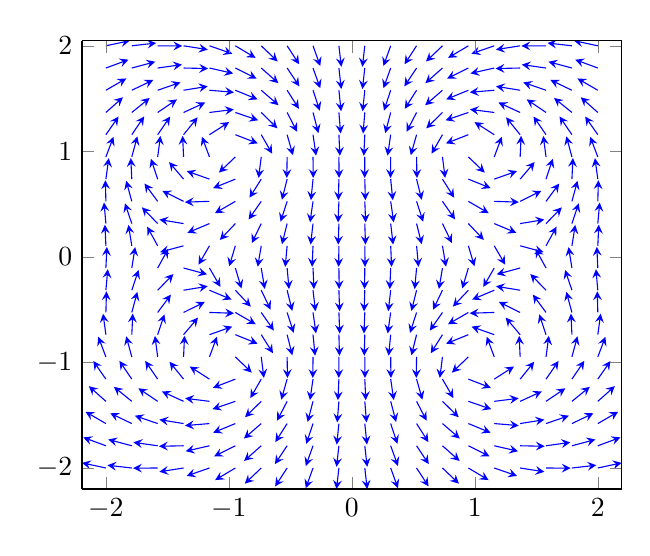
\begin{tikzpicture}
  \begin{axis}[
    domain=-2:2,
    view={0}{90},
    axis background/.style={fill=white},
  ]
    \addplot3[blue,
      quiver={
       u={
((y+1)/((x+1)^2+(y+1)^2)
+(y-1)/((x+1)^2+(y-1)^2)
-(y+1)/((x-1)^2+(y+1)^2)
+(-y+1)/((x-1)^2+(y-1)^2)
)
/
(sqrt(
(((y+1)/((x+1)^2+(y+1)^2)
+(y-1)/((x+1)^2+(y-1)^2)
-(y+1)/((x-1)^2+(y+1)^2)
+(-y+1)/((x-1)^2+(y-1)^2)
))^2
+((
-(x+1)/((x+1)^2+(y+1)^2)
-((x+1))/((x+1)^2+(y-1)^2)
+(x-1)/((x-1)^2+(y+1)^2)
+((x-1))/((x-1)^2+(y-1)^2)
))^2
))},
v={(
-(x+1)/((x+1)^2+(y+1)^2)
-((x+1))/((x+1)^2+(y-1)^2)
+(x-1)/((x-1)^2+(y+1)^2)
+((x-1))/((x-1)^2+(y-1)^2)
)
/
(sqrt(
(((y+1)/((x+1)^2+(y+1)^2)
+(y-1)/((x+1)^2+(y-1)^2)
-(y+1)/((x-1)^2+(y+1)^2)
+(-y+1)/((x-1)^2+(y-1)^2)
)
)^2
+((
-(x+1)/((x+1)^2+(y+1)^2)
-((x+1))/((x+1)^2+(y-1)^2)
+(x-1)/((x-1)^2+(y+1)^2)
+((x-1))/((x-1)^2+(y-1)^2)
))^2
))},
       scale arrows=0.2,
      },
      -stealth,samples=20]
        {1};
  \end{axis}
\end{tikzpicture}
\caption{B-Feld der Helmholzspulen.}
\label{fig:Skizze1}
\end{figure}

\item 

\begin{figure}[htbp]
\centering
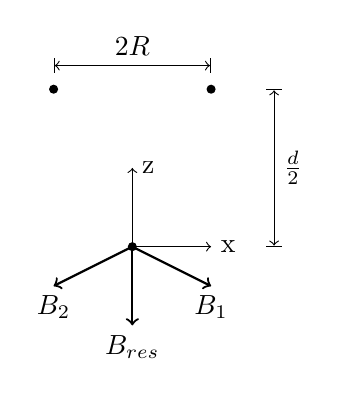
\begin{tikzpicture}


\filldraw (1,2) circle (0.05cm);
\filldraw (-1,2) circle (0.05cm);
\filldraw (0,0) circle (0.05cm);
\draw[->,thick] (0,0)--(1,-1/2);
\draw (1,-1/2) node[below] {$B_{1}$};
\draw[->,thick] (0,0)--(-1,-1/2);
\draw (-1,-1/2) node[below] {$B_{2}$};
\draw[->,thick] (0,0)--(0,-1);
\draw (0,-1) node[below] {$B_{res}$};

\draw[->] (0,0)--(0,1);
\draw (0,1) node[right] {z};
\draw[->] (0,0)--(1,0);
\draw (1,0) node[right] {x};

\draw[|<->|] (1.8,0)--(1.8,2);
\draw (1.8,1) node[right] {$\frac{d}{2}$};
\draw[|<->|] (-1,2.3)--(1,2.3);
\draw (0,2.3) node[above] {$2R$};


\end{tikzpicture}
\caption{B-Feld der Helmholzspulen.}
\label{fig:same}
\end{figure}

\item Das Feld einer Leiterschleife ergibt sich mit Hilfe des Biot-Savart-Gesetzes als 
\begin{equation}
  B(z)=\frac{I\mu_0}{2}\frac{R^2}{\left(R^2+z^2\right)^{\frac{3}{2}}}.
\end{equation}
Damit ist das Gesamtfeld gegeben durch
\begin{equation}
    B(z)=\frac{I\mu_0}{2}R^2\left(\frac{1}{\left(R^2+(z- \frac{d}{2})^2\right)^{\frac{3}{2}}}+\frac{1}{\left(R^2+(z+ \frac{d}{2})^2\right)^{\frac{3}{2}}}\right)
\end{equation}

\item 
  Für die zweite Ableitung des B-Feldes (auf der z-Achse) ergibt sich
\begin{equation*}
  \frac{\partial^2B_z}{\partial z^2}=\frac{I\mu_0}{2}R^2\left(\frac{15(\frac{d}{2}-z)^2}{(R^2+(z- \frac{d}{2})^2)^{\frac{7}{2}}}+\frac{15(\frac{d}{2}+z)^2}{(R^2+(z+ \frac{d}{2})^2)^{\frac{7}{2}}}-\frac{3}{(R^2+(z- \frac{d}{2})^2)^{\frac{5}{2}}}-\frac{3}{(R^2+(z+ \frac{d}{2})^2)^{\frac{5}{2}}}\right)
\end{equation*}
setzt man $z=0$ und form um erhält man schließlich $R=d$.

\end{enumerate}



